\documentclass{scrartcl}
\usepackage{tikz}
\usetikzlibrary{arrows,automata}
\usepackage{comment}

\begin{document}

% this is a single line comment and wont appear in the final document

% following block within \begin{comment} and \end{comment} are also comments;
\begin{comment}
NFA is defined as below and drawn pictorially

Hints:
- for set symbol, use \{ and \}
- for subscript $q_0$
- $ sets up math mode and you end with $
- also when you use special symbols such as _, ^, | etc, then use \$ to
  bracket them
- if $ doesnt match with another $, you will get warnings
- for math symbols, use \delta, \sum, \epsilon etc.
- for more symbols see http://www.artofproblemsolving.com/wiki/index.php?title=LaTeX:Symbols
- use \\ to denote new line
- for defining table, 
  - ||c c c|| defines 3 columns and so on
  - each row values are separated by &
  - use \space if you want to omit a column
- for drawing the DFA, we use tikz package
  - first 3 lines define the states, which one is initial, final etc
  - far right (eg. {$q_1$} will be drawn in the diagram within the circle
  - q1, q2, etc are like local variables used to define the machine
    and the transitions
  - you can specify how you want the arrows to look like--experiment
\end{comment}

Below is the NFA $M_1$ defined on Page 54 of the ITC \\
textbook. \\

% begin math mode with leading \$
$
Q = \{q_1, q_2, q_3, q_4 \} \\
\sum = \{0, 1 \} \\
F = \{q_4 \} \\
q_0 = q_1 \\
\delta = \{
			((q_1, 0), \{q_1\}), ((q_1, 1), \{q_1, q_2\}), ((q_1, \epsilon), \phi), \\
			((q_2, 0), \{q_3\}), ((q_2, 1), \phi), ((q_2, \epsilon), \{q_3\}), 		\\
			((q_3, 0), \phi), ((q_3, 1), \{q_4\}), ((q_3, \epsilon), \phi), 		\\
			((q_4, 0), \{q_4\}), ((q_4, 1), \{q_4\}), ((q_4, \epsilon), \phi)
		\}	\\
$
% end math mode with trailing \$

Transition Function in Table form: \\

% NFA Table representation

\begin{center}
 \begin{tabular}{||c c c c||} 
 \hline
 \space 	& 0 			& 1 				& $\epsilon$	\\ [0.5ex] 
 \hline
 $q_1$ 		& \{$q_1$\} 	& \{$q_1$, $q_2$\} 	& $\phi$		\\
 \hline
 $q_2$ 		& \{$q_3$\} 	& $\phi$  			& \{$q_3$\}		\\
 \hline
 $q_3$ 		& $\phi$ 			& \{$q_4$\} 	& $\phi$		\\
 \hline
 $q_4$ 		& \{$q_4$\} 	& \{$q_4$\} 		& $\phi$		\\
 \hline
\end{tabular}
\end{center}

NFA in Pictorial form: \\

% NFA pictorial representation

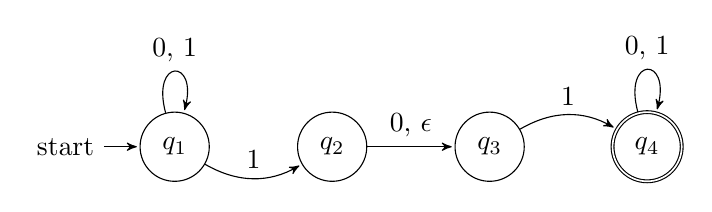
\begin{tikzpicture}[>=stealth',shorten >=1pt,auto,node distance=2cm]
  \node[initial,state	] 	(q1)      			{$q_1$};
  \node[state]  			(q2) [right of=q1]	{$q_2$};
  \node[state]         		(q3) [right of=q2] {$q_3$};
  \node[state, accepting]  (q4) [right of=q3] {$q_4$};

  \path[->] (q1) edge [loop above] 	node {0, 1} (q1)
             	 edge [bend right]     node {1} 	(q2)
        (q2) edge 				  		node {0, $\epsilon$} 	(q3)
        (q3) edge [bend left]  		node {1} 	(q4)
        (q4) edge [loop above] 		node {0, 1} (q4);
\end{tikzpicture}
\end{document}